\documentclass[border=4pt]{standalone}
\usepackage[T1]{fontenc}
\usepackage{helvet}
\renewcommand{\familydefault}{\sfdefault}
\usepackage{sfmath}
\hyphenpenalty=10000 \exhyphenpenalty=10000
\usepackage{amsmath}
\usepackage{tikz}
\usetikzlibrary{positioning,arrows.meta,fit,backgrounds}
\definecolor{ink}{HTML}{0B0B0B}\definecolor{sec}{HTML}{52514E}\definecolor{line}{HTML}{C3C2B7}
\definecolor{dev}{HTML}{2A78D6}\definecolor{thr}{HTML}{EB6834}\definecolor{tst}{HTML}{1BAF7A}
\definecolor{panel}{HTML}{F4F3F0}
\begin{document}
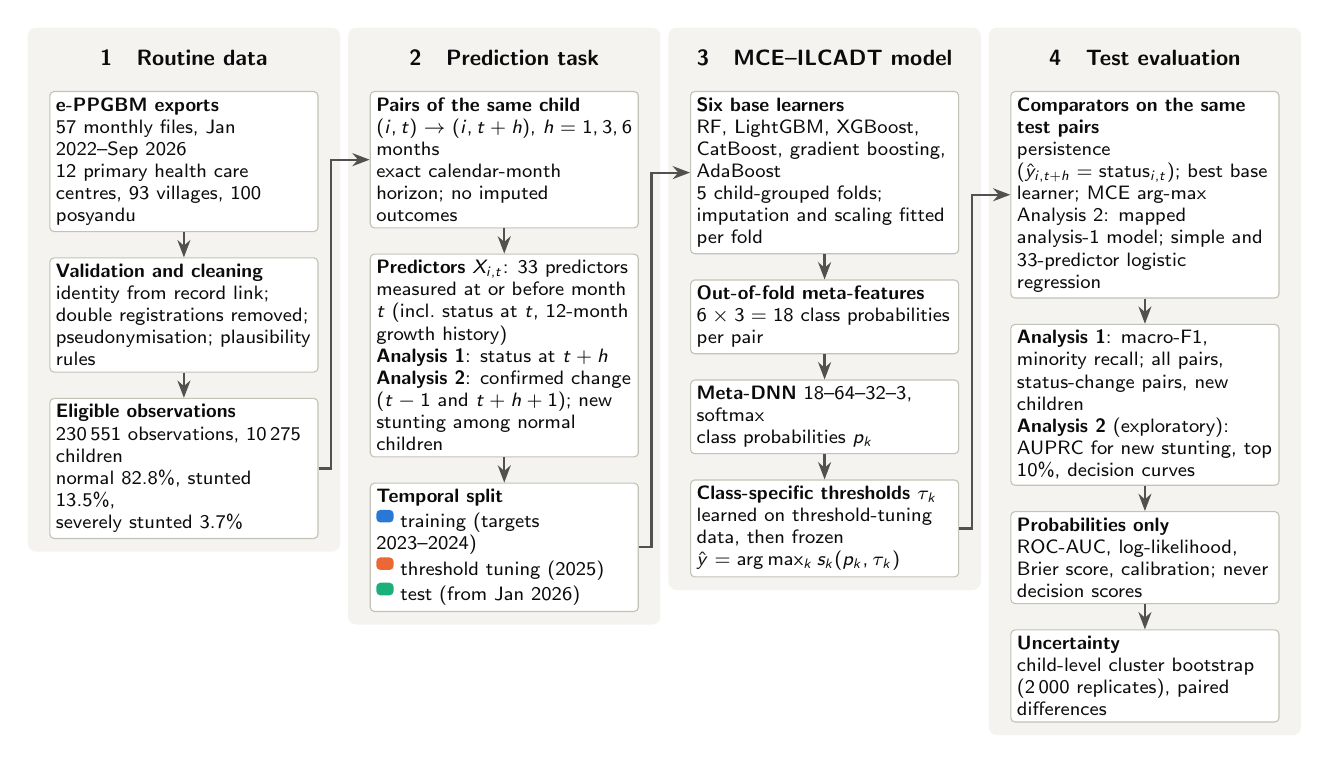
\begin{tikzpicture}[
  font=\scriptsize, node distance=3.2mm,
  box/.style={draw=line, fill=white, rounded corners=1.5pt, text width=32.5mm, align=flush left, inner sep=2.2pt, text=ink},
  hd/.style={font=\footnotesize\bfseries, text=ink, align=center, text width=34mm},
  arr/.style={-{Stealth[length=2.2mm]}, line width=0.8pt, draw=sec},
]
% ---------------- column 1: data
\node[hd] (h1) {1\quad Routine data};
\node[box, below=2mm of h1] (a1) {\textbf{e-PPGBM exports}\\ 57 monthly files, Jan 2022--Sep 2026\\ 12 primary health care centres, 93 villages, 100 posyandu};
\node[box, below=of a1] (a2) {\textbf{Validation and cleaning}\\ identity from record link; double registrations removed; pseudonymisation; plausibility rules};
\node[box, below=of a2] (a3) {\textbf{Eligible observations}\\ 230\,551 observations, 10\,275 children\\ normal 82.8\%, stunted 13.5\%,\\ severely stunted 3.7\%};
% ---------------- column 2: task
\node[hd, right=4.2mm of h1] (h2) {2\quad Prediction task};
\node[box, below=2mm of h2] (b1) {\textbf{Pairs of the same child}\\ $(i,t)\rightarrow(i,t+h)$, $h=1,3,6$ months\\ exact calendar-month horizon; no imputed outcomes};
\node[box, below=of b1] (b2) {\textbf{Predictors} $X_{i,t}$: 33 predictors measured at or before month $t$ (incl.\ status at $t$, 12-month growth history)\\ \textbf{Analysis 1}: status at $t+h$\\ \textbf{Analysis 2}: confirmed change ($t-1$ and $t+h+1$); new stunting among normal children};
\node[box, below=of b2] (b3) {\textbf{Temporal split}\\[1pt]
 \tikz[baseline=-0.6ex]\fill[dev] (0,0) rectangle (2.2mm,1.6mm); training (targets 2023--2024)\\
 \tikz[baseline=-0.6ex]\fill[thr] (0,0) rectangle (2.2mm,1.6mm); threshold tuning (2025)\\
 \tikz[baseline=-0.6ex]\fill[tst] (0,0) rectangle (2.2mm,1.6mm); test (from Jan 2026)};
% ---------------- column 3: model
\node[hd, right=4.2mm of h2] (h3) {3\quad MCE--ILCADT model};
\node[box, below=2mm of h3] (c1) {\textbf{Six base learners}\\ RF, LightGBM, XGBoost, CatBoost, gradient boosting, AdaBoost\\ 5 child-grouped folds; imputation and scaling fitted per fold};
\node[box, below=of c1] (c2) {\textbf{Out-of-fold meta-features}\\ $6 \times 3 = 18$ class probabilities per pair};
\node[box, below=of c2] (c3) {\textbf{Meta-DNN} 18--64--32--3, softmax\\ class probabilities $p_k$};
\node[box, below=of c3] (c4) {\textbf{Class-specific thresholds} $\tau_k$\\ learned on threshold-tuning data, then frozen\\ $\hat y=\arg\max_k s_k(p_k,\tau_k)$};
% ---------------- column 4: evaluation
\node[hd, right=4.2mm of h3] (h4) {4\quad Test evaluation};
\node[box, below=2mm of h4] (d1) {\textbf{Comparators on the same test pairs}\\ persistence ($\hat y_{i,t+h}=\text{status}_{i,t}$); best base learner; MCE arg-max\\ Analysis 2: mapped analysis-1 model; simple and 33-predictor logistic regression};
\node[box, below=of d1] (d2) {\textbf{Analysis 1}: macro-F1, minority recall; all pairs, status-change pairs, new children\\ \textbf{Analysis 2} (exploratory): AUPRC for new stunting, top 10\%, decision curves};
\node[box, below=of d2] (d3) {\textbf{Probabilities only}\\ ROC-AUC, log-likelihood, Brier score, calibration; never decision scores};
\node[box, below=of d3] (d4) {\textbf{Uncertainty}\\ child-level cluster bootstrap (2\,000 replicates), paired differences};
% ---------------- arrows
\draw[arr] (a1) -- (a2); \draw[arr] (a2) -- (a3);
\draw[arr] (b1) -- (b2); \draw[arr] (b2) -- (b3);
\draw[arr] (c1) -- (c2); \draw[arr] (c2) -- (c3); \draw[arr] (c3) -- (c4);
\draw[arr] (d1) -- (d2); \draw[arr] (d2) -- (d3); \draw[arr] (d3) -- (d4);
\draw[arr] (a3.east) -- ++(1.6mm,0) |- (b1.west);
\draw[arr] (b3.east) -- ++(1.6mm,0) |- (c1.west);
\draw[arr] (c4.east) -- ++(1.6mm,0) |- (d1.west);
% ---------------- background panels
\begin{scope}[on background layer]
\foreach \h/\l in {h1/a3,h2/b3,h3/c4,h4/d4}{\node[fill=panel, rounded corners=3pt, inner sep=1.6mm, fit=(\h)(\l)] {};}
\end{scope}
\end{tikzpicture}
\end{document}
